\documentclass[tikz,border=6pt]{standalone}
% Shared visual language for the book's standalone vector figures.
% Keep this file compatible with the TeX Live version used by LyX.
\usepackage{amsmath,amssymb}
\usepackage{array,booktabs}
\usepackage{pgfplots}
\usepackage{pgfplotstable}
\usetikzlibrary{arrows.meta,calc,positioning}
\pgfplotsset{compat=1.17}

\definecolor{BookBlue}{HTML}{0072B2}
\definecolor{BookOrange}{HTML}{D55E00}
\definecolor{BookGreen}{HTML}{009E73}
\definecolor{BookGray}{HTML}{666666}
\definecolor{BookLightGray}{HTML}{D9D9D9}

\pgfplotsset{
  book axis/.style={
    axis line style={black!75,line width=0.55pt},
    tick style={black!75,line width=0.45pt},
    tick label style={font=\small},
    label style={font=\small},
    legend style={
      font=\small,
      draw=none,
      fill=none,
      cells={anchor=west},
    },
    grid style={BookLightGray,line width=0.35pt},
    major grid style={BookLightGray,line width=0.35pt},
  },
}

\begin{document}
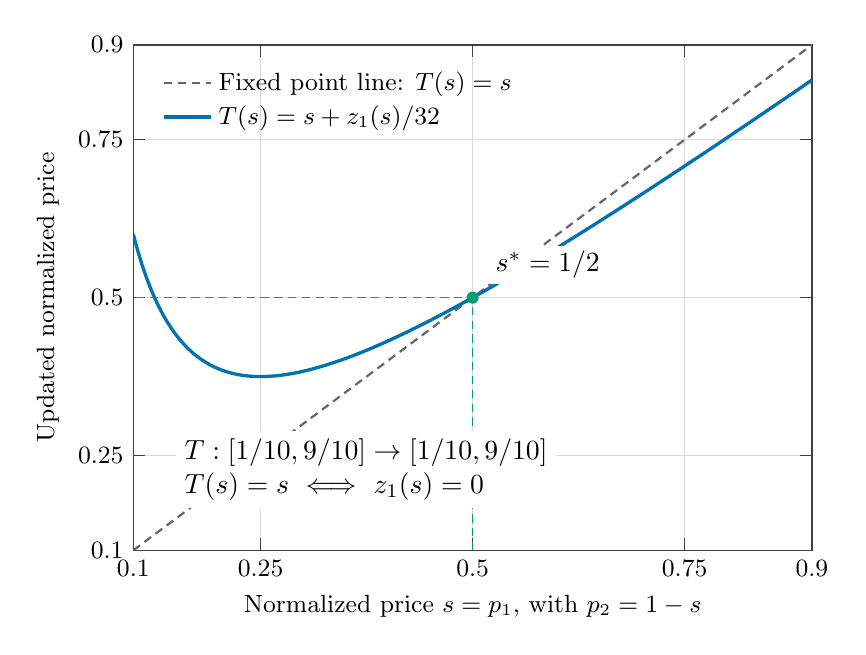
\begin{tikzpicture}
\begin{axis}[book axis,width=10.2cm,height=8cm,xmin=.1,xmax=.9,ymin=.1,ymax=.9,
 xlabel={Normalized price $s=p_1$, with $p_2=1-s$},ylabel={Updated normalized price},
 xtick={.1,.25,.5,.75,.9},ytick={.1,.25,.5,.75,.9},grid=major,
 legend style={at={(.03,.97)},anchor=north west}]
 \addplot[BookGray,densely dashed,thick,domain=.1:.9] {x};
 \addlegendentry{Fixed point line: $T(s)=s$}
 \addplot[BookBlue,very thick,domain=.1:.9,samples=160] {x+1/(16*x)-1/8};
 \addlegendentry{$T(s)=s+z_1(s)/32$}
 \draw[BookGreen,densely dashed] (axis cs:.5,.1)--(axis cs:.5,.5)--(axis cs:.1,.5);
 \fill[BookGreen] (axis cs:.5,.5) circle(2.2pt);
 \node[anchor=south west,fill=white,inner sep=2pt] at(axis cs:.52,.52){$s^*=1/2$};
 \node[anchor=north west,fill=white,inner sep=3pt,align=left] at(axis cs:.15,.29)
 {$T:[1/10,9/10]\to[1/10,9/10]$\\$T(s)=s\ \Longleftrightarrow\ z_1(s)=0$};
\end{axis}
\end{tikzpicture}
\end{document}
